\chapter{Adding Rodinia to Vortex}

One of \Gls{vortex}' weaknesses is its benchmark suite. Vortex includes only a few benchmarks, all of which are quite small and which behaviours does not match real-world applications. When lacking reasonable benchmarks, it is difficult obtain conclusive results about the performance of \Gls{vortex}. To solve this, I brought Rodinia~\cite{rodinia, rodinia_characterization}, a commonly used set of benchmarks for parallel computing~\cite{cactus}, to the Vortex ecosystem. This chapter describes the work done to enable Rodinia benchmarks to run on \Gls{vortex}. 

%\textcolor{red}{Vortex only has a few benchmarks. These programs have quite simple kernels and does not represent the behaviour of real world applications. Rodinia\cite{rodinia}\cite{rodinia_characterization} is a commonly used set of benchmarks for parallel computing \cite{cactus} with an OpenCL version. This chapter describes the work done to run Rodinia benchmarks on \Gls{vortex}}

\section{Reading Performance Data} \label{sec:reading_perf}

All the benchmarks included with \Gls{vortex} execute one kernel once. The existing setup for gathering performance data, created by the \Gls{vortex} team, took advantage of this. \Gls{vortex} utilize internal performance counters to collect performance data. Each \acrshort{sm} has its own counters, which are accessible as addressable \acrshort{csr} registers. Before a kernel is enqueued, the GPU and the performance registers are reset. After the reset, the kernel begins executing. Throughout the execution, different metrics are collected and stored in the \acrshort{csr} registers. When an \acrshort{sm} finishes the execution of its allocated workload, it ends by reading the relevant \acrshort{csr} registers and writing their contents to memory. The code related to dumping the performance counter to memory is included in every kernel by a stub. At the end of the benchmark, the host can read the memory, and collect the performance metrics for each of the \acrshortpl{sm}, and the \acrshort{gpu} as a whole.

Most of the benchmarks in Rodinia have more than one kernel, or execute a single kernel multiple times. When executing a multi-kernel benchmark, only the last execution would be recorded, because the \acrshort{gpu} would reset between kernel executions. Obtaining performance data for all kernels in a benchmark is important as they might possess radically different behaviours. An example of this would be the \textit{streamcluster} benchmark which has two kernels: \textit{memset} and \textit{pgain}. The memset kernel sets global memory to a given value. This results in a short loop and many writes to memory. The pgain kernel is more complex, having multiple branches, loops, calculations and memory operations. As the kernels are so different, it is important to capture the behaviour of both to be representative of the benchmark's performance.

The method used to read the performance data also has other issues which affect the accuracy and performance of the simulation.
\begin{enumerate}
    \item The process of reading performance registers and writing data to memory, alters the results while reading. The performance metrics read first, will not represent the same state as the ones read last.
    \item If \acrshortpl{sm} does not finish at the same time, performance metrics are written to memory while other \acrshortpl{sm} are running. Writing to memory may reduce the available memory bandwidth for the remaining cores.
    \item For programs running multiple kernels, or a single kernel multiple times, it is unnecessary to write the data to memory at the end of each kernel. This is especially significant when using software simulation, as it increases the simulation time.
\end{enumerate}

To solve these problems, I had to stop the performance metrics from being reset between kernel executions, and only collect performance metrics at appropriate times. To do this, I introduced two new CSR registers: \textit{perf-lock} and \textit{perf-reset-lock}. Setting \textit{perf-lock} stops the collection of performance metrics. When \textit{perf-reset-lock} is set, the performance metrics are not reset when the \acrshort{gpu} resets. However, as \textit{perf-reset-lock} controls what is reset, it cannot be controlled by reset itself. To ensure the performance metrics are reset before starting the benchmark, I have to first execute a kernel to specifically set the lock low. This solves the problem of benchmarking multiple kernels. 

Problems 2 and 3 listed above, can be resolved by moving the code responsible for writing the performance data to memory, into a separate kernel which is executed after the benchmark has been completed. Doing this makes sure that all of the \acrshortpl{sm} complete their workloads before starting the process of reading performance data. The kernel reading the performance data, sets the \textit{perf-lock} to ensure that it does not interfere with the data while reading, thus also solving problem~1. 

The final solution, illustrated in Figure \ref{fig:init_run_dump}, can be divided into three phases. \textcircled{\small{1}} Before starting the execution of a benchmark, the initializing kernel is executed. It is responsible for setting the \textit{perf-reset-lock} low, to allow the performance metrics to reset correctly. \textcircled{\small{2}} The kernels belonging to the benchmark are then executed. They also set the \textit{perf-reset-lock} high, to keep the data from resetting. The benchmark continues to execute its kernels until it has been completed. \textcircled{\small{3}} Finally, the performance dump kernel is executed, setting the \textit{perf-lock} high to stop it from altering the results.

\begin{figure}
    \centering
    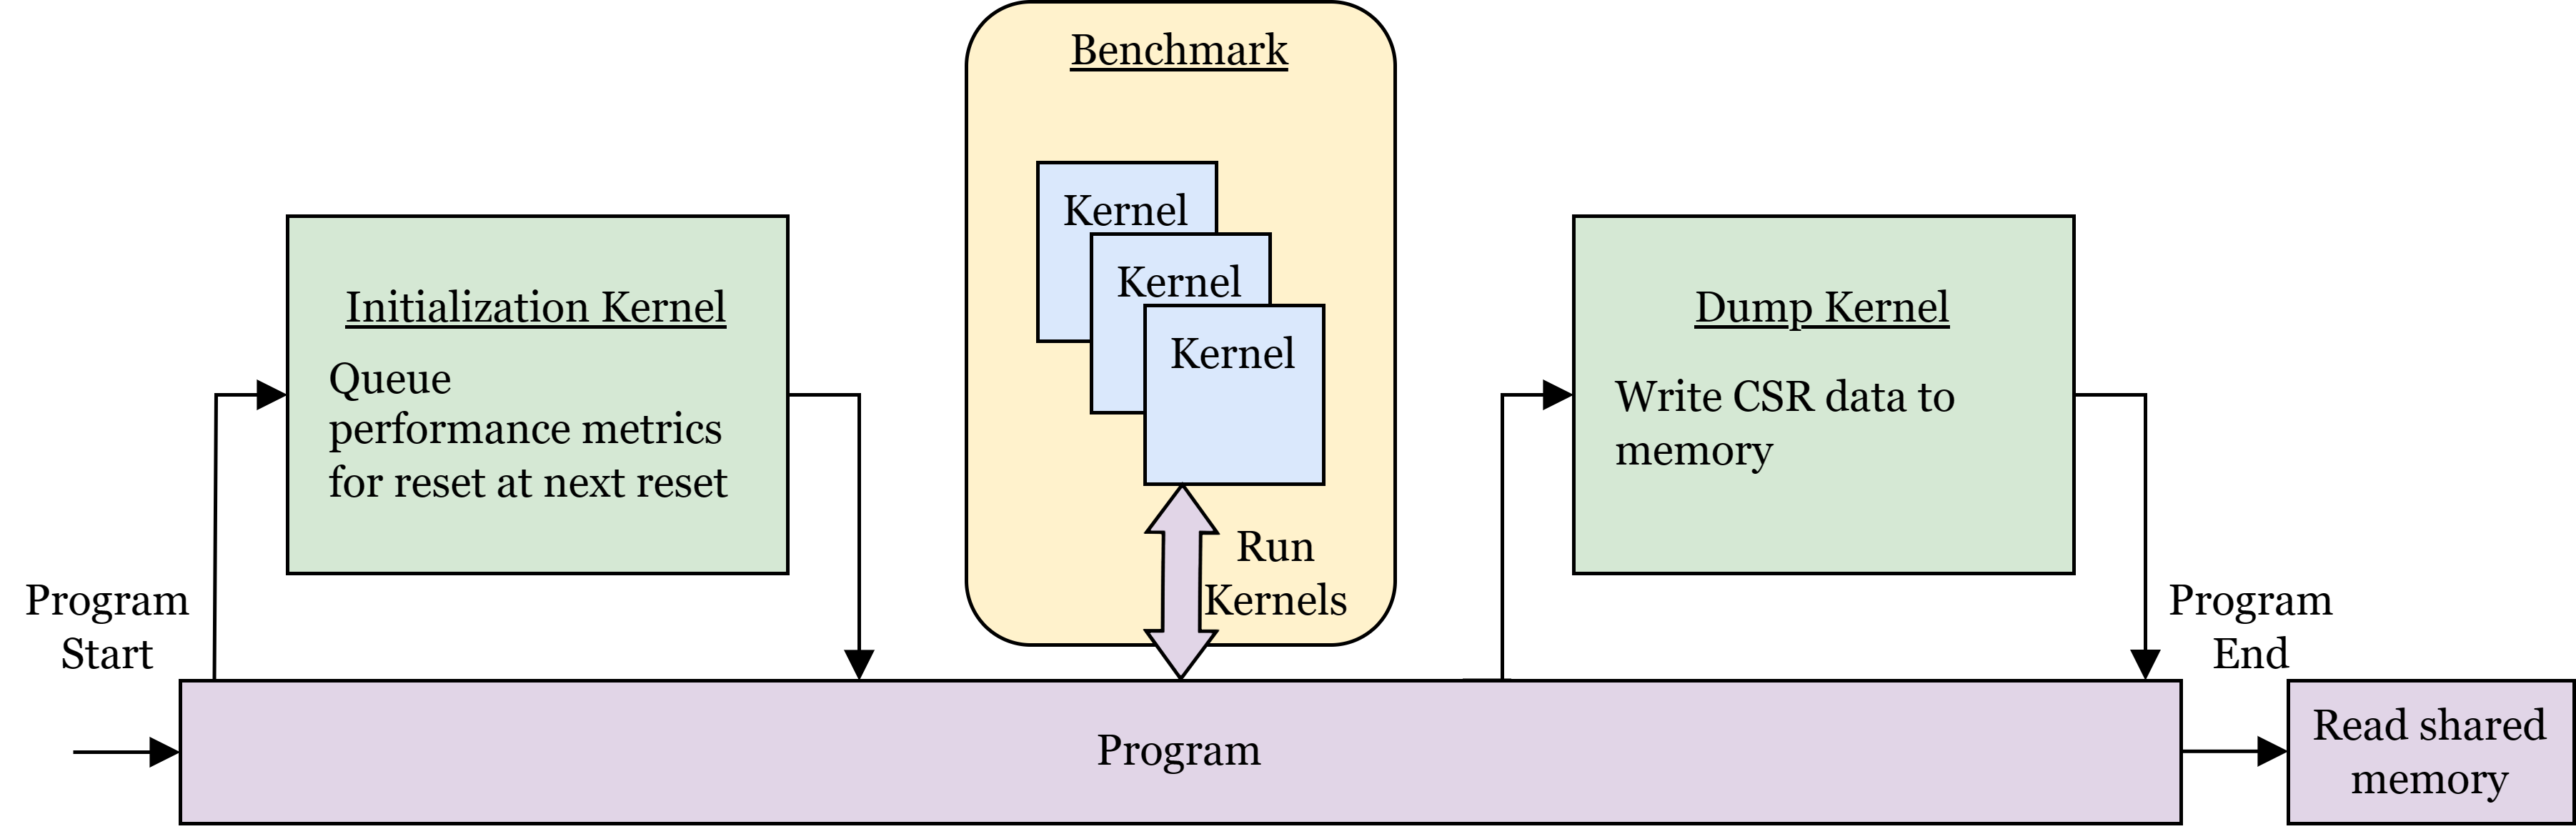
\includegraphics[width=\textwidth]{figures/perf-kernels.png}
    \caption[Timeline of the three stages of multi-kernel benchmarking.]{Timeline of the three stages of multi-kernel benchmarking: \textit{initialization}, \textit{execution of benchmark} and \textit{dumping of performance data}}
    \label{fig:init_run_dump}
\end{figure}

To make this solution viable to implement for all benchmarks, I created a header file, containing macros for creating and starting the two new kernels. To add new benchmarks to \Gls{vortex}, it is only required to include the header and insert the macros at the correct location. The macros take the current OpenCL context, command queue and device ID as input. An example snippet of how this can be used is shown in Code~listing~\ref{lst:macros}. Doing this allowed for more rapid adjustments to the implementation, in addition to making the process of adding new benchmarks quicker.

\begin{lstlisting}[language=C, caption=Example of using the perf macros to create and use the initialization and dump kernels, label={lst:macros}]
#include "../vortex_perf.h"             // Header containing perf macros

PERF_VARIABLES // Macro declaring variables required to run perf kernels

// -- Code for setting up OpenCL: create context, command-queue and device

PERF_CREATE_PROGRAM(context, device_id) // Macro for creating the perf kernels
PERF_ENQUEUE_INIT_KERNEL(command_queue) // Macro for starting the init kernel

// -- Code for running the benchmark

PERF_ENQUEUE_DUMP_KERNEL(command_queue) // Macro for starting the dump kernel
PERF_CLEANUP                            // Macro for perf kernel cleanup 
\end{lstlisting}

\section{Adapting Benchmarks for Vortex}

When simulating \Gls{vortex} in software, Verilator~\cite{verilator} is used to compile the SystemVerilog implementation of \Gls{vortex} into a vortex library. This library can simulate the entire \acrshort{gpu} cycle-accurately. When executing a benchmark, it is linked with the \Gls{vortex} driver and \Gls{vortex} library generated by Verilator. This allows the host to treat the simulated \acrshort{gpu} as if it was a normal \acrshort{gpu} using an OpenCL interface. The software and \acrshort{fpga} simulations thus provide the same interface. Because of this, the changes done in this section should also work for \acrshort{fpga}-accelerated simulations.

\newpage
\subsection{Offline Compilation}

\Gls{vortex} has support for OpenCL, and uses \gls{pocl}~\cite{pocl} to implement the compiler and runtime software, which provides an OpenCL interface for the host. The compiler has been modified to support the generation of kernel binaries targeting the extended \Gls{riscv} \acrshort{isa} used by \Gls{vortex}. The \gls{pocl} driver does however not support online compilation. Thus all kernels have to be compiled offline and loaded as binaries. This means that variables can not be passed from the program to the kernel before compilation. Because of this, the buffer sizes of some of the benchmarks had to be hard-coded, instead of changing with the input of the benchmark. This makes the benchmarks less flexible.

The \textit{hybridsort} and \textit{myocyte} benchmarks from \Gls{rodinia} have kernels which require specific functions. This includes \texttt{atomic\_add}, \texttt{expd}, \textit{powdd} and \texttt{sqrtd}. These functions were missing from the \Gls{pocl} compiler. These benchmarks could therefore not be included in \Gls{vortex}' benchmark suite. After further inspections, it became apparent that none of the atomic functions are included by the \Gls{pocl} compiler. 

\subsection{Memory Allocation}

While porting \Gls{rodinia} benchmarks to \Gls{vortex}, I observed that the OpenCL functions \texttt{clEnqueueNDKernels}, \texttt{clEnqueueCopyBuffer} and \textit{clCreateBuffer} sometimes aborted or resulted in segmentation faults. Looking into the cause of the crashes, I found that \texttt{clEnqueueNDKernels} caused a segmentation fault when the kernel contained local parameters. It seems like the driver is unable to dynamically allocate local memory for the \acrshortpl{tb} using \texttt{clSetKernelArg}. To solve this, I removed the local parameters of the kernels, and instead defined local buffers in the kernel code. By doing this, the driver does not have to allocate the buffers dynamically. As the size of the local buffers is now defined at compile time of the kernels, I had to hard-code the buffer sizes according with the selected input of the benchmarks.

The \texttt{clCreateBuffer} function creates a buffer on the \acrshort{gpu} to store data. If the \texttt{GL\_MEM\_ALLOC\_HOST\_PTR} flag of \texttt{clCreateBuffer} is set, the allocated memory should be accessible by the host. For \Gls{vortex} it seems like using this flag results in a segmentation fault. To resolve this, I instead created the buffer without the flag, and used \texttt{clEnqueueReadBuffer} and \texttt{clEnqueueWriteBuffer} to access the memory whenever needed by the host. This issue is similar to the one above, as it seems to be caused by issues regarding the permission to dynamically allocate memory in specific locations.

The last OpenCL function I encountered issues with was \texttt{clEnqueueCopyBuffer}. \texttt{clEnqueueCopyBuffer} copies data from one buffer on the \acrshort{gpu} to another. I is unclear why this is causing a crash, but it could be easily resolved by reading the data from the device to the host using \texttt{clEnqueueReadBuffer}, before writing it back to the destination buffer using \texttt{clEnqueueWriteBuffer}. The workarounds described in this  using the problematic OpenCL features should not affect the measured performance, as measurements are made only during kernel execution.

\subsection{Selecting Work Sizes}

Table~\ref{tab:new_benchmarks} shows the list of Rodinia benchmarks which can execute on \Gls{vortex} after performing the adaptations mentioned in this section. However, the benchmarks were not scheduled efficiently, by \Gls{vortex}' static \acrshort{tb} scheduler. The scheduler struggled to divide the work among \Gls{vortex}' \acrshortpl{sm}. For most benchmarks only a small subset of the \acrshortpl{sm} were scheduled any work. Rekdal~\cite{Rekdal_Master} encountered the same issue with some of the existing \Gls{vortex} benchmarks. The solution was to reduce the local work size to 1 when enqueuing the kernels. This reduces the number of threads per \acrshort{tb}, resulting in more \acrshort{tb}, which can be scheduled to more \acrshortpl{sm}. This method worked to some degree for all benchmarks except \textit{heart wall}, which I was unable to improve upon.  

% -- Table of benchmarks
\begin{table}
    \centering
    \caption{Rodinia benchmarks added to \Gls{vortex}}
    \begin{tabular}{|l|l|l|l|} 
        \hline
        \textbf{Applications}      & \textbf{Domains} \\ \hhline{|=|=|}
        B+ Tree                    & Graph Traversal \\ \hline
        Back propagation           & Pattern Recognition \\ \hline
        Breadth-First Search       & Graph Algorithms  \\ \hline
        CFD Solver                 & Fluid Dynamics  \\ \hline
        Gaussian elimination       & Linear Algebra \\ \hline
        GPUDWT                     & Image/Video Compression  \\ \hline
        Heart Wall                 & Medical Imaging \\ \hline
        HotSpot                    & Physics Simulation  \\ \hline
        HotSpot3D                  & Physics Simulation  \\ \hline
        Kmeans                     & Data Mining \\ \hline
        LavaMD2                    & Molecular Dynamics\\ \hline
        LU Decomposition           & Linear Algebra  \\ \hline
        Needleman-Wunsch           & Bioinformatics\\ \hline
        Particle Filter            & Medical Imaging \\ \hline
        SRAD                       & Image Processing  \\ \hline
        Streamcluster              & Data Mining \\ \hline
    \end{tabular}
    \label{tab:new_benchmarks}
\end{table}

\section{Fast-Forward, Warm-Up and Early-Exit} \label{sec:ff_wu_ee}

Most of the added Rodinia benchmarks require substantially more time to complete execution than the already included benchmarks. When using software simulation, it becomes infeasible to simulate the entire benchmarks, due to long simulation times. One way of solving this would be to reduce the input sizes, however, this would affect the TB scheduler and cache behaviour. A more common approach for reducing simulation time is using \textit{fast-forwarding} and \textit{warm-up}~\cite{simpoint}. Fast-forwarding is to run a less accurate simulation to a given point in execution, and then continue the real simulation from there. This skips the initialization, and samples only the part of the code most representative of the whole benchmark. After fast-forwarding using a less accurate simulator, branch predictors and caches will not be in the same state as if an accurate simulation was used. A solution is to then run the accurate simulation until the cache hit rate stabilizes, before collecting performance metrics. This is called warm-up and removes the cold-start bias.

There is no emulator or less accurate simulator for \Gls{vortex}, thus fast-forwarding and warm-up will have limited versatility. To further reduce simulation time, I introduce \textit{early-exit} to \Gls{vortex}. Early-exit terminates the benchmark after a given number of cycles. As the number of simulated cycles scales linearly with the simulation time, early-exit allows me to easily regulate the simulation time. When implementing early-exit, it becomes more important to skip the startup, i.e. using fast-forward and warm-up, as it becomes a larger portion of the execution time. Figure~\ref{fig:ff-timeline} illustrates how fast-forward, warm-up and early-exit affect which execution cycles are sampled.

\begin{figure}
    \centering
    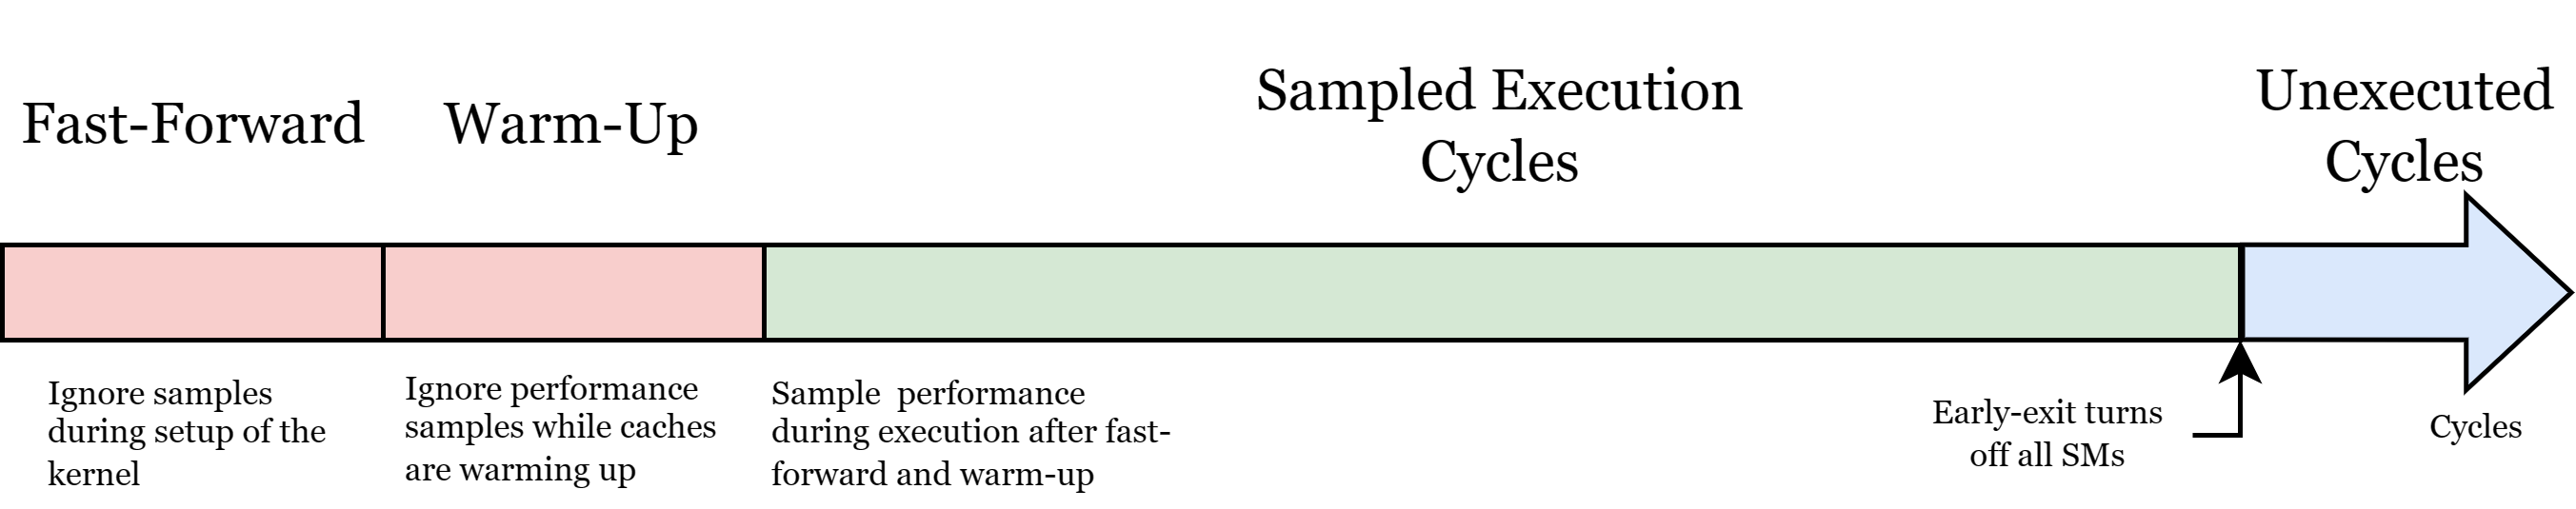
\includegraphics[width=\textwidth]{figures/fast-forward-timeline.png}
    \caption{Timeline explaining fast-forward, warm-up and early-exit.}
    \label{fig:ff-timeline}
\end{figure}

Fast-forward and warm-up are implemented by setting the \textit{perf-lock} register, described in Section \ref{sec:reading_perf}, high for a given number of cycles at the beginning of the simulation. Thus no performance data will be collected during the startup. Caches and other components can also be warmed during this period. Note that this is only performed for the first kernel in a benchmark. If a benchmark executes multiple kernels before exiting, the startup cycles become representative of the kernel's performance. Early-exit is implemented by deactivating all the \acrshortpl{sm} after a given number of cycles. This indicates to the driver that \Gls{vortex} has completed its execution. 

This method of implementing early-exit is somewhat problematic. When terminating early, the result of the kernels will not be correct. Some of the benchmarks are affected by the results returned by the kernel execution. \textit{Streamcluster} does for example execute the kernel until the result is not getting better. If the result is wrong due to early-exit, it might result in an infinite loop of starting and exiting the kernel. To resolve this, I had to manually add safeguards for \textit{streamcluster} and \textit{kmeans}, setting a maximum number of iterations.
